\documentclass[../main.tex]{subfiles}
\begin{document}

\tags{
    \nameref{hc:audience},
    \nameref{hc:distributions},
    \nameref{hc:gapanalysis},
    \nameref{hc:medium},
    \nameref{hc:sampling},
    \nameref{hc:variables}
}{
    \LOref{CausalBenchmarkTheory},
    \LOref{CausalBenchmarkDesign},
    \LOref{CausalProblemSpace},
    \LOref{GraphicalModels}
}

The remainder of this paper is focused on Maccabee. Maccabee - \textbf{M}onte \textbf{C}arlo \textbf{Ca}usal \textbf{Be}nchmarks using \textbf{E}mpirical data - is a Python Package that makes Hybrid Monte Carlo benchmarking available to researchers and practitioners. This chapter provides a formal description of Maccabee's benchmarking approach. The next chapter presents the implementation of this design.

\vspace{\baselineskip}

As noted at the end of Chapter \ref{chap:litreview}, the design described here builds on the theoretical design proposed in \textcite{Dorie2019Automated1}, extending it into a flexible, implementation-ready \textit{concrete} design. The concrete design is presented in four sections. The first section provides a brief summary of the methods reviewed in Chapter \ref{chap:litreview}. This sets the context that informed the design proposed in this chapter. The second section outlines Maccabee's benchmarking approach. First, looking at the high-level approach used by \textcite{Dorie2019Automated1} and then at how this approach is concretized in Maccabee's DGP sampling procedure. The third section provides a formal statistical specification of a Maccabee benchmark. The fourth section outlines how Maccabee measures the location of sampled DGPs in the distributional problem space from Chapter \ref{chap:problemspace}. Finally, the fifth section discusses the empirical data sets that are included in the package, as these form an important part of the `design' of a Hybrid Monte Carlo benchmark. Taken together, the content of these four sections provides a complete picture of the design of the Maccabee package.

\section{Design Goal: Better Benchmarking for Causal Inference Methods}
\label{mac:problems}

As established in Chapter \ref{chap:litreview}, most existing approaches to benchmarking methods for causal inference fall into one of two \textit{pure} design categories:

\begin{enumerate}
    \item \textbf{Empirical methods} use real, observed covariate and outcome data. This data is typically drawn from randomized experiments so that ground truth effect values are known (although experiments only provide average effect estimates). In these benchmarks, there is a true Data Generating Process (DGP) but it is latent and its properties are unknown. It is unclear if the data meets the typically required causal inference assumptions, especially after modifications like replacing the random control group with non-random data to create a \textit{psuedo-observational} setting in which randomization, and the resultant expected covariate balance, doesn't hold.

    \item \textbf{Synthetic methods} use covariate and outcome data generated from synthetic (hand-specified rather as opposed to observed/empirical) distributions and functions. By definition, the DGP is known. As a result, the true causal effects - both at the average and individual level - can be calculated directly and it is known if causal assumptions are met.
\end{enumerate}

While both of these approaches have strengths and weaknesses, explored in detail in Chapter \ref{chap:litreview}, they share a common flaw: their sample size is, effectively, one. In either design, a new causal inference method is tested against one or a few DGP (per targeted distributional setting). In empirical datasets, the properties of this DGP and, most importantly, its place in the distributional problem space, are unknown. The causal inference method is validated against a single DGP `sample' from an unknown location in the problem space. In synthetic datasets, the DGP properties - and its location in problem space - are known but, again, there is usually only one or a few DGPs per distributional setting.

\vspace{\baselineskip}

In the best case, either of these approaches risks missing important aspects of estimator performance in the selected region of problem space by failing to average over variance in performance present in structurally similar DGPs. In the worst case, the results are biased - either by the failure of empirical data to conform to basic causal assumptions or by manual specification using unrealistic data or unrepresentative/simplistic versions of DGP from the selected region (unintentionally). In either scenario, benchmarking results are unlikely to generalize as indicators of consistent, real-world performance.

\vspace{\baselineskip}

The primary design goal of the Maccabee is to enable a benchmarking approach that mitigates the flaws of the common approaches analyzed above. This is done by adopting the theoretical design proposed by \textcite{Dorie2019Automated1}.

\section{Approach: Flexible, Reusable Hybrid Benchmarking}
\label{mac:approach}

This section outlines Maccabee's benchmarking approach. The high-level approach is inspired by, and closely follows, the benchmarking process proposed in \textcite{Dorie2019Automated1}. The low-level design specifics of the approach, and the corresponding implementation described in Chapter \ref{chap:macimplementation}, are de novo.

\subsection{Dorie et al's Approach to Hybrid Benchmarking}
\label{mac:generalapproach}

The benchmarking process proposed by \textcite{Dorie2019Automated1} mitigates the weaknesses outlined in Section \ref{mac:problems} by \textit{sampling} Data Generating Processes. This approach has enormous potential usefulness because sampled DGPs have treatment/outcome mechanisms defined over arbitrary covariates (arbitrary empirical data) and sampled from parameterized distributions over a subspace of functions. With the parameterization of these distributions allowing for control over the expected location of sampled DGPs in the distributional problem space (established in Chapter \ref{chap:problemspace}). This approach allows for:

\begin{itemize}
    \item More thorough exploration of the distributional problem space (relative to empirical benchmarks) because DGPs can be sampled from many different (known) locations in the problem space. Methods designed to tackle specific classes of distributional settings can be tested on these settings.

    \item More realistic covariate distributions (relative to synthetic benchmarks) because sampled DGPs can (but do not have to) consist of sampling functions defined over empirical/observed sets of covariate data. The flexibility of the sampling process means that almost any empirical data can be used, allowing methods to be tested on the kind of data they are designed to handle in real applications.

    \item More robust results (relative to either of the pure approach) because performance evaluations are performed by averaging across many DGPs selected, in a principled manner, from a region of problem space.
\end{itemize}

The problem is that the concrete design, implementation and validation presented by \textcite{Dorie2019Automated1} are tied to a single data set and set of sampling parameters. Maccabee is designed to mitigate these weaknesses. But, before getting into the specifics of how this is achieved, it is important to establish the components of \textcite{Dorie2019Automated1}'s abstract design that are adopted by Maccabee.

Following \textcite{Dorie2019Automated1}, the core workflow in Maccabee samples a treatment assignment, an untreated outcome function, and a treatment effect function and then uses these functions as the components $\Omega$, $\Phi$ and $\tau$ to concretize the generic DGP outlined in Chapter \ref{chap:litreview}. The sampled functions are drawn from the subspace of \textit{generalized, additive functions} - additive functions with terms that are 1st, 2nd, or 3rd-degree polynomials, two or three-way interactions, and linear functions with jump discontinuities in their value or derivative.

\vspace{\baselineskip}

The fourth degree of freedom in the concretization process - the joint distribution over covariates, $\rho$ - is specified to be either an empirical distribution over observed covariates or an arbitrary joint distribution. In either case, the three sampled functions are defined over the covariates from $\rho$.

\subsection{Concretizing Dorie et al.'s Approach}

\subsubsection{Departure Point}

While the approach described above makes sense, it does not prescribe a specific sampling scheme and associated set of sampling parameters that could be used to sample DGPs from a desired location in the distribution problem space. \textcite{Dorie2019Automated1} do, in fact, propose such a scheme and even supply an R implementation (available \href{https://github.com/vdorie/aciccomp}{here}). The problem is that this scheme and implementation is designed to generate a static set of benchmarking datasets - using a single empirical covariate dataset and a single set of sampling parameterizations. Further, the code is not designed to execute benchmarks or perform metric calculation; it is only designed to generate a single static set of benchmarking data. Finally, the code is poorly documented which makes parsing (and modifying) the exact parameterization used by the authors a non-trivial, specially for method developers not familiar with Hybrid Benchmarking and focused on their own research.

\vspace{\baselineskip}

Maccabee proposes its own parameterization and sampling scheme, based on the general approach outlined above. This scheme is then implemented such that it can be used with any covariate data and with arbitrary, easy-to-specify parameterizations. It is designed to allow users to use their own empirical data, easily specify locations in the distributional problem space, and run repeated benchmarks using new, dynamically generated data sets.

\subsubsection{Maccabee's Approach}

The goal of the explanation below is to show how a set of \textit{DGP Sampling Parameters} can be used to sampled DGPs from a region of the distributional problem space. As established in Chapter \ref{chap:problemspace}, this means the parameters must (approximately) control the location of sampled DGPs along the seven problem space axes. Discussion of how sampled DGPs can then be used to implement benchmarking is covered in the formal specification in Section \ref{mac:formalspec}.

\vspace{\baselineskip}

In Maccabee, the distribution over functions is central to this control. Sampled DGP functions are made up of the linear combination of the set of \textit{term types} listed in Section \ref{mac:generalapproach} above. These term types are 1st, 2nd, or 3rd-degree polynomials, two or three-way interactions, and linear functions with jump discontinuities in their value or derivative. Covariates may appear in multiple terms, so the \textit{universe} of concrete terms for each \textit{term type} is all of the combinations of covariates that could appear in the form of the \textit{term type} (there are some restrictions, noted below). The distribution over the functions is specified by the set of (uniform) probabilities that each term in the universe of terms for each term type \textit{term type} is selected to appear in the function. This means the function distribution is parameterized by seven probability parameters, one per \textit{term type}. In addition to this, each term has a co-efficient sampled from a co-efficient distribution. While this distribution is central to the Maccabee design, the complete DGP sampling procedure must be complicated to allow for control over the complete set of axes.

\vspace{\baselineskip}

The procedure is given below. The parameters which influence the operation of each step are given in bold at the end of each step description.

\begin{enumerate}
    \item A set of \textit{potential confounders} is selected from all of the covariates based on a single, uniform selection probability. This is the set of confounders that could enter either/both of the sampled treatment/outcome mechanisms. Fewer selected covariates produce a lower signal-to-noise ratio in the data and, therefore, makes the modeling of the treatment/outcome mechanisms harder. \label{proc:confounders}

    \item The treatment assignment and untreated outcome functions are sampled from two independently parameterized distributions of the kind described above. The universe of each \textit{term type} is specified by the combination of all the potential confounders selected in step \ref{proc:confounders}. The coefficients in all of the terms of two functions are initialized by drawing samples from a parameterized, global, co-efficient distribution.

    \vspace{\baselineskip}

    Note that, in the generic DGP described in Chapter \ref{chap:litreview}, the treatment assignment is sampled using a single function referred to as $\Omega$. In this concretization, $\Omega$ is split into a treatment probability and treatment assignment function. The treatment probability function is sampled in the manner described above and the treatment assignment produces assignments conditioned on the probability. For simplicity, this difference is not made explicit in the explanations below.

    \item An alignment (confounding) adjustment is performed. This step involves randomly selecting terms to add/remove from the sampled treatment assignment and untreated outcome functions to meet a target alignment parameter. This parameter specifies the target probability for a term in the untreated outcome function to also appear in the treatment assignment function. Lower alignment thus implies a more disjoint set of covariates appearing across the functions. This produces weaker confounding of the treatment assignment and outcome variables present in the generated data.

    \item The treatment effect mechanism is then sampled. First, a constant treatment effect is sampled from a parameterized, global treatment effect distribution. Then, terms from the untreated outcome function are sampled based on a treatment effect heterogeneity parameter. This parameter specifies the uniform probability that a term in the untreated outcome function appears in the treatment effect function. This means the treatment effect function can be thought of as a subset of the untreated outcome function terms (plus a constant offset) that interact linearly with the binary treatment assignment.

    \item Numerical normalization and linear modification (by multiplicative/additive constants) of the treatment assignment function is used to meet target parameters for the min/expected/max value of the treatment probability

    \item Numerical normalization and linear modification (by multiplicative/additive constants) of the untreated outcome function is applied to adjust the signal-to-noise ratio of the observed outcome. This is an automatic adjustment without parameterization.

    \item Finally, some components of the DGP sampling only occur at data generation time. On each instance of data generation:

    \begin{enumerate}
        \item A fixed proportion of the covariates are sampled with the default being that all observations are sampled. This step can be used to mimic small datasets (or heavy, at-random censorship) when using empirical datasets. This will change the number of observations in each generated dataset.
        \item Observed outcome noise is sampled from a parameterized, global outcome noise distribution.
        \item A parameterized target proportion of the units in the treated and control groups with the lowest/highest probability of treatment respectively are swapped between the groups. This creates a larger imbalance in the covariate distribution between the groups.
    \end{enumerate}

\end{enumerate}

By controlling the probability with which different term types appear in the treatment assignment, untreated outcome, and treatment effect functions, as well as the overlap of terms between the functions, one can (approximately) control linearity, degree of confounding, and causal effect heterogeneity. By controlling the distributions from which the treatment effect, outcome noise, and constant coefficients are sampled, and applying normalization techniques, one can (approximately) control the location and scale distribution over outcome values and probabilities of treatment (as well as the signal-to-noise ratio of these quantities with respect to the covariates). Finally, by swapping units between groups, one can (approximately) control the imbalance in the distribution of covariates across the treated/control groups.

\vspace{\baselineskip}

Note that the degrees of freedom listed above correspond exactly to the axes that make up the distributional problem space. Therefore, by using the parameters that control these degrees of freedom, it is possible to generate DGPs that are - in expectation - located in different regions of the space. This, in turn, allows for better evaluation of new causal inference methods. Both by evaluating them across more regions in the problem space and more robustly in each region by sampling multiple, structurally similar DGPs and averaging out any function-specific effects.

\section{Formal Specification of the Maccabee Benchmark}
\label{mac:formalspec}

Section \ref{mac:approach} above provided an overview of the approach taken by Maccabee, focusing on the DGP sampling procedure. This section provides a formal specification of the end-to-end benchmarking procedure. The specification takes the form of a statistical model, depicted as a graphical model, that describes a complete Maccabee Monte Carlo benchmark. The DGP sampling procedure from the previous section is only a sub-component of the statistical model depicted here.

\subsection{Statistical Model}

Figure \ref{fig:mac-graph-model} contains a graphical model that provides a formal, statistical description of Maccabee's benchmarking process. It explicates the relations between all of the (fixed) parameters and (sampled) random variables that are combined to produce a benchmark result (a Monte Carlo estimate of one or more metric defined over the estimand sampling distribution). This can be thought of as a description of the benchmarking process at the level of data that is completely generic with respect to the functions/distributions that relate/produce the data.

\vspace{\baselineskip}

It is important to note that this model extends (and slightly modifies) the generic DGP statistical model proposed in Chapter \ref{chap:litreview} (as well as the concretized, sampled-function version from Section \ref{mac:approach}). Those models included only the \textit{DGP Random Variables} (and the relations between them). The model below extends this set of variables to include \textit{Estimand Random Variables}: The causal estimand random variables - samples from the estimand sampling distribution - and the performance metrics calculated over this distribution. As well as the data metrics that quantify the position of the DGP in the distributional problem space. Three notational tools are used to make this extension:

\begin{itemize}
    \item \textit{DGP Random Variables} - that are part of the original generic DGP framework - are indicated in white while \textit{Estimate Random Variables} - either estimands or metrics derived from these estimates - are in blue.

    \item Plate notation is used to indicate that each dataset includes $N$ observations and that $M$ such datasets, each drawn from a different DGP - are present in the benchmark described by the model. Each dataset has an associated set of performance and data metrics (that are themselves random variables). There is one metric value (for each metric) per dataset.

    \item The $DGP$ random variable - sampled based on the \textit{DGP Sampling Parameters} - represents the treatment and outcome mechanisms that connect the observed covariates to the *oracle* (latent/unobserved) treatment and outcome random variables. This variable stretches graphical notation, so it worth a brief discussion.

    \vspace{\baselineskip}

    Ordinarily, the functions/distributions relating the covariate variable $X$ to the treatment/outcome variables would be represented by the edges between these variables - each defined by fixed, parametric functional forms. In the Maccabee benchmarks, these functions/distributions are themselves sampled based on underlying parameters and distributions. As such, they are best represented as a Random Variable which conditions the value of the random variables that are related/generated by the DGP. The single $DGP$ random variable can thus be thought of as a variable that abstracts lower-level functional detail.

\end{itemize}

Finally, it is worth noting that the estimator used to generate average/individual causal effect estimates from the observed outcome data is not explicitly depicted in this model. This estimator - whether stochastic or deterministic - is represented by the edges connecting the observed DGP variables to the individual/average estimate values.

\begin{figure}[ht!]
    \centering
    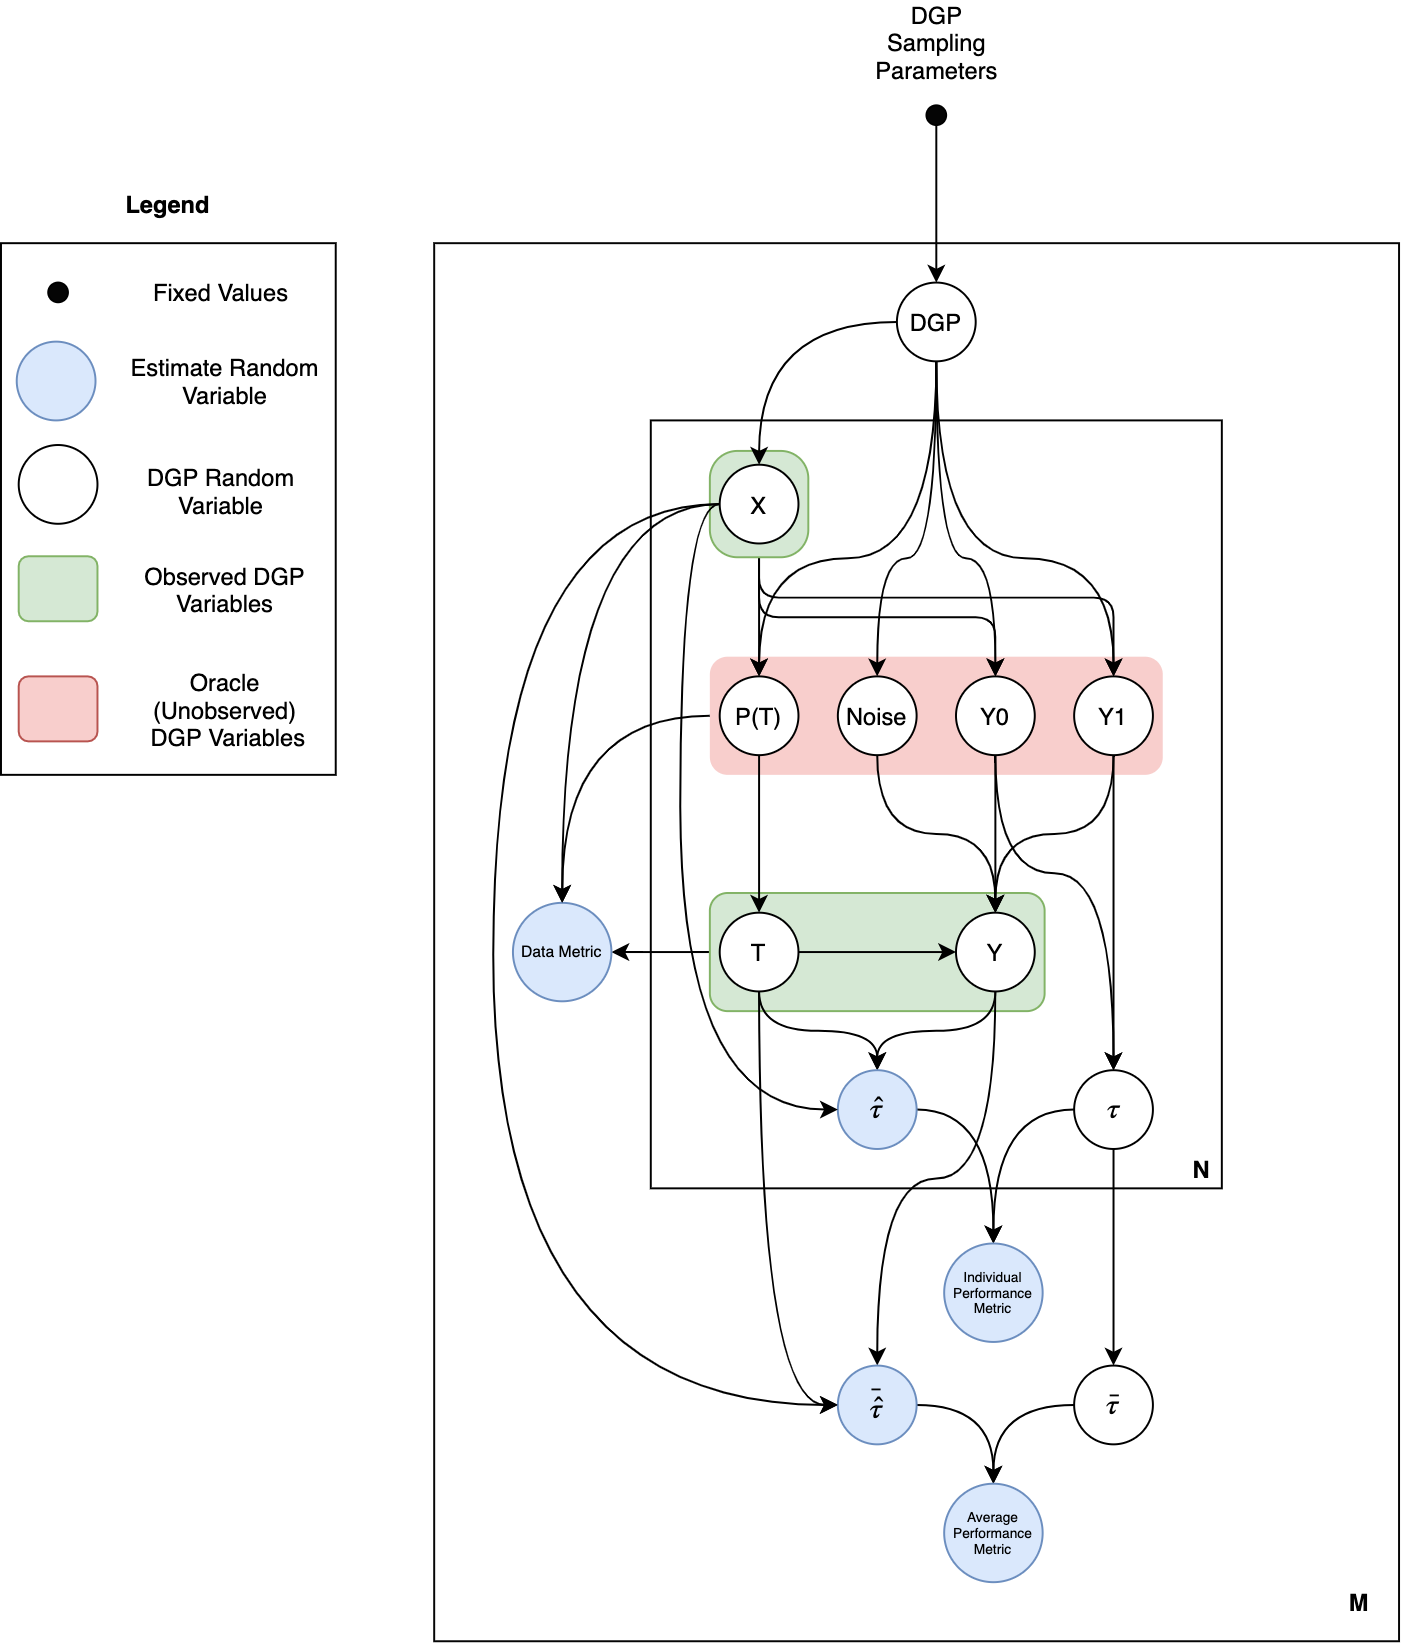
\includegraphics[width=1\linewidth]{figures/ch5-maccabee-design-graphical-model-fig.png}
    \caption{A Graphical Model depicting the complete statistical model of the a Maccabee Monte Carlo benchmark.}
    \label{fig:mac-graph-model}
\end{figure}
\FloatBarrier

\subsection{Sampling Procedure}

The graphical model in Figure \ref{fig:mac-graph-model} concretely specifies the sampling procedure used to execute a Maccabee Monte Carlo benchmark. Moving from the top of the model to the bottom:

\begin{enumerate}

\item A set of $M$ DGPs is sampled from a distribution parameterized by the fixed \textit{DGP Sampling Parameters} described above.

\item A set of $N$ covariate observations - each represented by the variable $X$ - is drawn for each $DGP$ (actually from the subcomponent of the DGP representing the joint distribution over covariate observations, the $\rho$ distribution in the theory paper).

\item Each covariate observation $X$ has an associated set of treatment assignment, outcome, and causal effect random variables. Added to the observed covariates, these variables represent the complete observed and unobserved information about each individual observation in the dataset. Following the nomenclature from Chapter \ref{chap:problemspace}, I interchangeably refer to unobserved variables as oracle variables.

\vspace{\baselineskip}

Note that, for expositional clarity, the dependencies between the individual observation variables depicted in this model are slightly different from the actual relations implied by the sampled DGPs described in Section \ref{mac:formalspec} above.

\vspace{\baselineskip}

With that established, the sampling procedure for each individual observation is given below:

\begin{itemize}
    \item The \textit{oracle} (unobserved) treatment probability ($P(T)$) is sampled conditioned on the covariate observation $X$ and the treatment probability function (defined over $X$) from the sampled $DGP$. The \textit{observed} treatment assignment - $T$ - is then sampled conditioned on $P(T)$.

    \item The \textit{oracle} (unobserved) potential outcome variables ($Y1$ and $Y0$) are sampled conditioned on the covariate observation $X$ and the outcome functions (defined over $X$) from the sampled $DGP$. This is true to Rubin's Potential Outcome framework as described in Chapter \ref{chap:framework} but is not in line with procedure implied by the structure of the sampled DGPs from Section \ref{mac:formalspec} above. In a sampled DGP, only the untreated outcome, $Y0$, is sampled (from the untreated outcome function, $\Phi$). This value is them combined with a treatment effect (sampled from the treatment effect function, $\tau$) to produce the treated outcome, $Y1$. This difference simplifies the graphical model and is irrelevant for the remainder of the sampling procedure.

   \item The \textit{oracle} (unobserved) outcome noise is sampled from the outcome noise distribution from the sampled $DGP$.

   \item The \textit{observed} outcome variable - $Y$ - is sampled conditioned on the treatment assignment, potential outcomes, and outcome noise.

   \item The individual causal effect variable - $\tau$ - is (deterministically) sampled conditioned on the potential outcome variables. Note, again, that in the sampled DGP, the individual treatment effect is sampled from the treatment effect function, $\tau$.

\end{itemize}

\item Causal estimand values can be sampled at the individual observation or dataset level. At the individual level, $N$ individual effect estimates $\hat{\tau}$ are sampled from a (deterministic/stochastic) estimator conditioned on each $X$, $T$ and $Y$. At the dataset level, a single average effect estimand $\bar{\hat{\tau}}$ is sampled from a (deterministic/stochastic) estimator conditioned on all $N$ of the $X$, $T$ and $Y$ observations.

\item Following estimand sampling, $M$ Individual or Average Performance Metric values are calculated (deterministically sampled) at the dataset level by combining the causal effect estimate values with the appropriate ground-truth value(s) - $\tau$ or $\bar{\tau}$ respectively.

\item Finally, and optionally, $M$ Data Metrics are calculated by combining some/all of the covariate data with the observed and oracle outcome data.

\end{enumerate}

\section{Measuring the Location of Sampled DGPs in the Distribution Problem Space}
\label{sec:measuring-distributional-setting}

\textcite{Dorie2019Automated1} propose the use of \textit{metrics}, defined over the various DGP variables discussed above, to measure the location of a DGP along an axis. These metrics work by assigning a numerical `score' to data drawn from a DGP, such that this score is proportional (in some approximate way) to the property described by the target axis. Note that these metrics are, therefore, \textit{estimates} of the position along an axis for two reasons. First, the metric itself is only \textit{proportional} to the underlying axis \textit{concept} and there may be many, roughly equivalent functions that share this proportionality property but do not produce values that are absolutely comparable. Second, the metric value is calculated using data sampled from the DGP. This means there is sampling variance associated with the metric value. That said, it is not crucial that these metrics are perfectly `accurate' because there is ground truth against which the accuracy of the metric can actually be measured. The distribution problem space is a \textit{conceptual} design space. Estimators are expected to be sensitive to the location of data/DGPs in this space, but it is the region of the data in the space more than the (undefinable) exact location that matters. This means heuristic/approximate metrics, that measure relative position, are acceptable and useful. Note that throughout the package implementation and documentation, the metrics introduced here are referred to as \textit{data metrics} and the metrics used to measure performance are referred to as \textit{performance metrics}. For simplicity, the rest of this section uses \textit{data metrics} and metrics interchangeably.

\vspace{\baselineskip}

With this established, I proceed to describe the metrics proposed by \textcite{Dorie2019Automated1}. These metrics can be used to measure all of the axes proposed above and are implemented directly in Maccabee. As is evident from the discussion in Chapter \ref{chap:macvalidation}, there are many aspects of the metric scheme that could be improved. These improvements are left to future work. 

\vspace{\baselineskip}

Rather than describe each of the metrics that appear in Maccabee, I focus on the methods used to measure \textit{concepts} that are common to the metrics used for multiple axes of the problem space. For example, the linearity of some variable with respect to another where linearity is the \textit{concept}. Before doing this, I first draw a distinction between the so-called \textit{oracle} and \textit{observed} variables over which the metrics are defined as well as introducing the notion of \textit{transformed covariates}. A complete list of the metrics proposed by \textcite{Dorie2019Automated1}, and implemented in Maccabee, can be found in the supplementary material of their paper.

\subsection{Observed vs Oracle Variables}

Chapter \ref{chap:problemspace} established that the axes of the distributional problem space correspond to properties of the distributional setting - the joint distribution over the observed data. This implies that the position of a DGP in the distributional problem space can by determined by the properties of the (observed) data generated by the DGP. While this is true, it is clear that distributions over the unobserved data/aspects of the DGP also play a critical role in creating/defining the distributional setting of the observed data. For example, the linearity of the outcome mechanism depends on the distribution over the potential outcome without treatment - $Y0$ - conditioned on the observed covariates.

\vspace{\baselineskip}

Accurate measurement of the position of observed data along the axes above, therefore, requires access to both observed and unobserved data. Without this access, it is still possible to \textit{approximately} measure the location, but it may be hard to disambiguate location along related axes (for the same reason that observational causal inference is hard in the first place). For example, low linearity of the observed outcome with respect to the covariates could imply non-linearity in the untreated outcome mechanism or the treatment effect mechanism. This doesn't mean that all metrics over observed data are approximate. For example, an estimate of the linearity of treatment assignment may be accurate given that both true treatment assignment and covariates are observed.

\vspace{\baselineskip}

If the true DGP is known, then one has access to both observed and unobserved variables. This means that metrics including both can be calculated. To draw a distinction between (sometimes inaccurate) metrics over observed data and (usually accurate) metrics over unobserved data, \textcite{Dorie2019Automated1} refer to the former as observed metrics and the later as oracle metrics. I adopt this nomenclature in the rest of the paper when referencing these classes of metrics and the variables they rely on.

\subsection{Original and Transformed Covariates}

\textit{Transformed covariates} are especially useful oracle variables (see the section above) that result from the design of the sampling scheme used in Maccabee. As described in \ref{mac:approach}, the treatment and outcome functions that are the core of Maccabee's sampled DGPs are constructed as a linear combination of non-linear transformations, each of which involves one to three observed covariates. The value of these non-linear transformations can be thought of as `covariates' that are related to the treatment and outcome by simple linear functions. This perspective is useful when constructing metrics that require controlling for the functional form of the treatment/outcome functions. Examples are discussed below. The values of the non-linear terms that make up the sampled functions are referred to as the \textit{transformed covariates} throughout the package implementation and documentation.

\subsection{Functions for Measuring Axes `Concepts'}

While the axes introduced in Chapter \ref{chap:problemspace} each correspond to a unique property of the distributional setting, there is a smaller number of unique \textit{concepts} that appear across the axes (and, accordingly, in the metrics used to measure the position of DGPs along the axes). For example, the concept of linearity appears directly in three of the axes (and indirectly in one more). The combination of a concept and the data to which the concept is applied forms a unique axis.

\vspace{\baselineskip}

Metrics that measure the position of data/DGPs along each axis are built using functions that measure these concepts (applied to the relevant subset of the observed/oracle variables). Below, I describe the three \textit{concepts} that constitute/cover all of the nontrivial metrics in \textcite{Dorie2019Automated1} and outline the different functions that can be used to produce quantified (but heuristic) estimates of each concept.

\begin{enumerate}
    \item \textbf{Linearity:} the linearity of the function which relates some (potentially vector-valued) variable $A$ to a real-valued variable $B$ can be quantified using the $R^2$ value of a linear regression of $B$ on $A$. This captures how much of the variance in $B$ can be explained through a linear relation with $A$. If $B$ is categorical, the linear regression can be replaced by a logistic regression to achieve the same effect in the probability space of the relationship between $A$ and $B$. Metrics that use this approach are applied to measure the axes:

    \begin{itemize}
        \item The Nonlinearity (Modeling Complexity) of the (Untreated) Outcome Mechanism
        \item The Nonlinearity (Modeling Complexity) of the Treatment Effect Mechanism
        \item The Nonlinearity/Complexity of the Treatment Assignment Mechanism
        \item The Degree of Alignment Between the Treatment Assignment and Outcome Mechanism \footnote{Measuring the correlation between the treatment and observed/oracle outcome variables can be used as a proxy for the ratio of confounding to non-confounding variables in the treatment and outcome mechanism}.
    \end{itemize}
    
    Measures of linearity can also be combined with the \textit{transformed covariates} to measure more specific aspects of modeling complexity. For example, a linear regression of the outcome without treatment onto the transformed covariates measures the impact of the outcome noise on outcome predictability. This is possible because, by using the transformed covariates, the linear regression is guaranteed to be based on the correct model specification. Ergo, any prediction error is from other sources of error - with outcome noise being the only other source in this case.

    \item \textbf{Distributional distance:} the distributional distance between two sets of observations of the same variables can be measured in a number of ways.
    \vspace{\baselineskip}
    \textbf{Mean-based Distance Measures}

    \begin{itemize}

        \item The L2 (vector-space) distance between the mean of variables in each set of observations. This approach summarizes each group of observations using the mean of each variable and then calculated the distance between the means. This is only useful if the mean is a good summary, and if the variables have roughly similar scales. Otherwise, a (relatively) small difference in the value of the mean of a variable with a (relatively) large scale may overwhelm all the very similar mean values of variables with small scales and produce a large overall distance.

        \item The Mahalanobis distance between the group means. This is equivalent to the L2 distance with each covariate scaled by its empirical standard deviation. This accounts for the scaling problem assuming the empirical standard deviation is an appropriate scale factor.
    \end{itemize}

    \textbf{Distribution-based Distance Measures}

    \begin{itemize}
        \item Both the L2 and Mahalanobis distance can be applied to nearest-neighbor pairs across the two sets of observations - rather than the mean - with the result averaged across the data set. This produces a measure of distributional similarity that doesn't rely on the mean summary and is empirically weighted by the number of observations in each region of the domain.

        \item The Wasserstein distance measures the absolute difference in the cumulative distribution function for the distribution across the domain. Conceptually, this is the amount of probability mass that would have to be moved in one of the distributions to equalize the two distributions.
    \end{itemize}

    Metrics that use the distance measures above are applied to measure the axes:

    \begin{itemize}
        \item Covariate Balance
        \item Covariate Distribution Overlap \footnote{It is impossible to know whether the distribution of the empirical data in the treatment groups overlaps, so distance measures at the distributional level are used as a proxy}
    \end{itemize}

    \item \textbf{Relative Heterogeneity}: the heterogeneity of some variable $A$, relative to another variable $B$, can be measured using the ratio of the standard deviation of $A$ to the standard deviation of $B$. Metrics that use this approach are applied to measure the axes:

    \begin{itemize}
        \item Treatment Effect Heterogeneity \footnote{The standard deviation in the treatment effect relative to the standard deviation in the untreated outcome measures can be used as a proxy for the heterogeneity in the treatment effect.}
    \end{itemize}
\end{enumerate}

\section{Empirical Data Sets in Maccabee}
\label{mac:data}

The sections above discuss the joint distribution over covariates, the $\rho$ component of the DGP, entirely generically. In reality, the selection and construction of this distribution is an important aspect of Maccabee's core design. As mentioned by section \ref{mac:generalapproach} above, and justified in Chapter \ref{chap:litreview}, the design advantage of Maccabee comes from the combination of \textit{empirical} covariates and sampled treatment and outcome mechanisms. This section discusses the use of empirical covariate distributions in Maccabee.

\vspace{\baselineskip}

As implied by the name, an empirical covariate distribution is a joint distribution over observed covariates with an unknown parameterization, ergo one which is defined, empirically, by the data itself. This data may be an incomplete/biased sample so that the empirical covariate distribution defined by it is not the same as its true underlying joint distribution.

\vspace{\baselineskip}

Maccabee is designed with both a set of included, high-quality empirical covariate distributions as well as tools to allow for the use of user-supplied data to define custom empirical covariate distributions. These two approaches are described in the sections below.

\subsection{Included Empirical Covariate Distributions}

Maccabee includes empirical covariate distributions defined by data sets from the literature on causal inference benchmarking. These data sets were selected because they are:

\begin{itemize}
    \item Used widely, indicating a social consensus that they are high quality - representative, useful - data sets for the evaluation of causal inference methods.

    \item Varied in the number of observations and covariates, allowing for benchmarking of methods under different circumstances.

    \item Open source, meaning the data can be accessed and used by others to ensure that any results reproduce as expected.
\end{itemize}

\subsubsection{The National Support Work (NSW) Data Set}

This is a data set corresponding to the NSW data, introduced by \textcite{Lalonde1986EvaluatingData}, that appears throughout the early causal inference literature. Building on \textcite{Dehejia2005PracticalTodd} and \textcite{Smith2005DoesEstimators}, the package uses a selected subset of the \textcite{Lalonde1986EvaluatingData} experimental data (the subset with real income in 1974 available) and the \textit{PSID} observational controls with the data downloaded from \href{https://users.nber.org/~rdehejia/data/.nswdata2.html}{here}. In the experimental data, there are 297 treated units and 425 control units. The control units are dropped in favor of the 2490 PSID units to produce a non-randomized observational setting \footnote{Note that, even though the treatment and outcome mechanisms will be sampled, it is necessary to drop the experimental controls to reproduce the covariate distributions in the Lalonde data set}. Real Income in 1978 is the measured outcome. All other variables are measured pre-treatment and serve as covariates.

\subsubsection{The Collaborative Perinatal Project (CPP) Data Set}

The CPP data set is extracted directly from the benchmarking implementation provided by \textcite{Dorie2019Automated1}. The authors describe the data set as follows.

\begin{quote}
    The Collaborative Perinatal Project (Niswander and Gordon, 1972), is a massive longitudinal study that was conducted on pregnant women and their children between 1959 to 1974 with the aim of identifying causal factors leading to developmental disorders. The publicly available data contains records of over 55,000 pregnancies, each with over 6500 variables. Variables were selected by considering a subset that might have been chosen for a plausible observational study. Given the nature of the dataset, we chose to consider a hypothetical twins study examining the impact of birth weight on a child’s IQ. We chose covariates that a researcher might have considered to be confounders for that research question. After reducing the data set to complete cases, 4802 observations and 58 covariates remained. Of these covariates, three are categorical, five are binary, 27 are count data and the remaining 23 are continuous.
\end{quote}


\subsection{Custom Empirical Covariate Distributions}

 In Maccabee, almost any data can be used to define an empirical covariate distribution. This is useful for benchmarking methods that are designed to work well in very specific covariate settings. The tools that enable the use of custom empirical data sets are described in the package documentation \RTDlink{here}.

 \vspace{\baselineskip}

 It is crucial to note that the properties of the sampled DGPs, measured along the axes from Chapter \ref{chap:problemspace}, are sensitive to the empirical covariate distribution. This means that, in order to produce DGPs in the desired region of the distributional problem space, it is usually necessary to both lightly pre-process the covariate data and fine-tune the other DGP sampling parameters. There are limits on how much of these two steps can be automated by the package. By default, Maccabee applies normalization to the covariates appropriate for pair-wise independent, symmetric distributions of each covariate. The default sampling parameters are also tuned to expect this form of distribution. If any other data is used, care will need to be taken. Fortunately, the formal metrics used to measure the position of sampled DGP in the distributional problem space can be used to guide this process without any fear of overfitting/compromising benchmark validity. DGP sampling is done prior to any causal estimation, so pre-processing and sampling parameter values can be adjusted until metric values indicate that DGP samples are being drawn from the desired region of the problem space.

\end{document}